\documentclass[12pt]{fphw}
%\usepackage{mathpazo}
%\usepackage[utf8]{inputenc}
%\usepackage[T1]{fontenc}
\usepackage{sectsty}
\usepackage{graphicx}
\usepackage{booktabs}
\usepackage{listings}
\usepackage{enumerate}
\usepackage{xcolor}

\sectionfont{\bfseries\large\raggedright}

\definecolor{codegreen}{rgb}{0,0.6,0}
\definecolor{codegray}{rgb}{0.5,0.5,0.5}
\definecolor{codepurple}{rgb}{0.58,0,0.82}
\definecolor{backcolour}{rgb}{0.95,0.95,0.92}

\title{Experiment 1}
\author{Aditya Kumar (24MAI14003)\\}
\date{06 Aug, 2024}
\institute{Chandigarh University\\Master of Engineeing---Artificial Intelligence}
\class{Advanced Python Programming (24CSH-623)\\}
\professor{Kirandeep Kaur}

\begin{document}

\maketitle

\section*{}
\begin{problem}
  \textbf{Aim: }Installation of Python and understanding of basic syntax and semantic rules.\\
  Write a python program to illustrate the concept of different types of operators.
\end{problem}
\section{Theory}
\subsection{Arithmetic Operators}
Used for mathematical operations like addition ($+$), subtraction ($-$), 
multiplication ($*$), division ($/$), modulo ($\%$), integer division ($//$), and exponentiation ($**$).
\subsection{Assignment Operators} 
Used to assign values to variables (e.g., $+=, -=, *=, /=$).
\subsection{Comparison Operators}
Used for comparing values (e.g., $==, !=, <>, >, >=, <, <=$). They return 
boolean results (`True` or `False`). 
\subsection{Logical Operators}
Used to combine conditional statements (e.g., and, or, not). 
\subsection{Bitwise Operators}
Used to perform bitwise operations on integer numbers (e.g., $\&, |, ^, ~, <<, >>$). 
\subsection{Identity Operators}
Identity Operators: Used to compare objects (e.g., is, is not). 
\subsection{Membership Operators}
Used to test whether a value is present in a sequence (e.g., in, not in).

\section{Code}
    \lstinputlisting[language=Python, backgroundcolor=\color{backcolour}, numbers=left, tabsize=2,basicstyle=\ttfamily\footnotesize, breaklines=true]{e1.py}
\section{Output}
  \begin{center}
    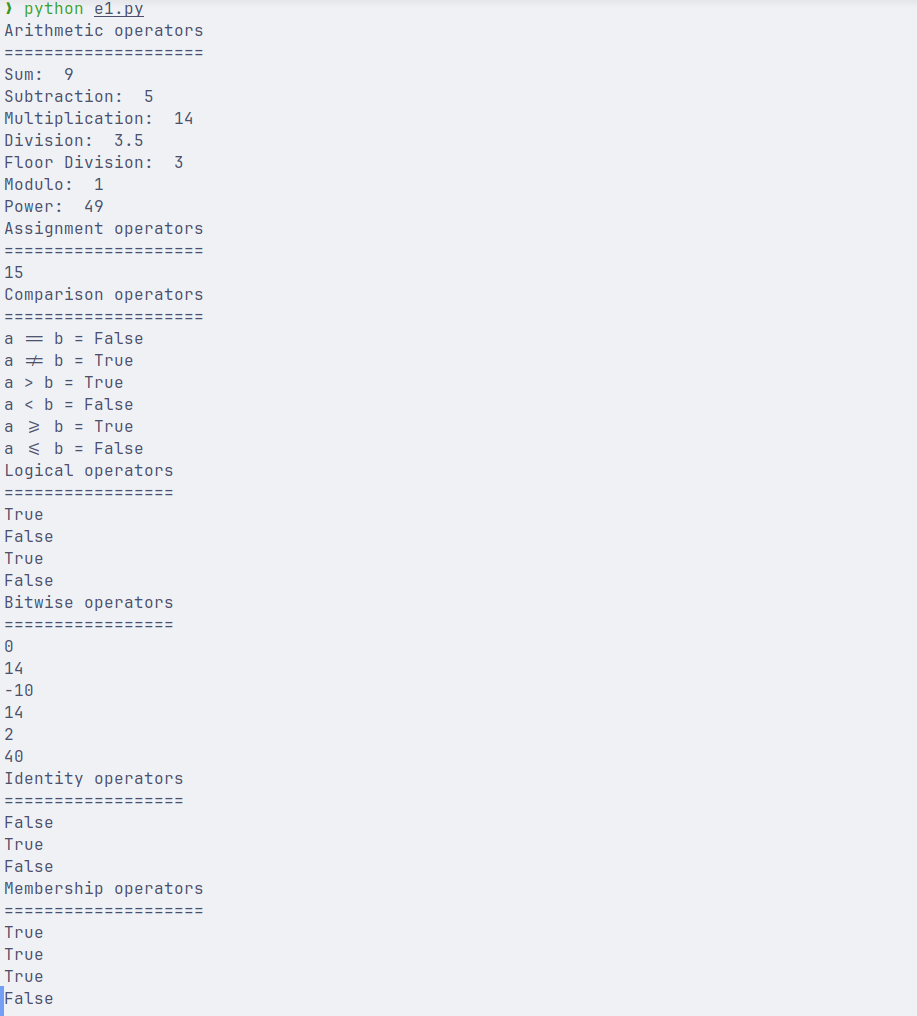
\includegraphics[width=0.7\columnwidth]{./e1.png}
  \end{center}
\section{Learning Outcomes}
Learnt about operators in Python.
\end{document}
